\documentclass[11pt]{article}
\usepackage[margin=1in]{geometry}
\usepackage{graphicx}
\usepackage{booktabs}
\usepackage{amsmath}
\usepackage{xcolor}
\usepackage{caption}
\usepackage[hidelinks]{hyperref}
\usepackage{titlesec}
\titleformat{\section}{\large\bfseries}{\thesection}{0.6em}{}
\captionsetup{font=small, labelfont=bf}
\definecolor{accent}{HTML}{B07D1F}

\title{\textbf{RateWalk: Forecasting Fed Rate Decisions with a Shrunk Markov Chain}\\[2pt]
\large An out-of-sample, point-in-time study of whether inflation regimes help}
\author{Tanishk Yadav\\\small MS Financial Engineering, New York University\\\small \texttt{tanishkyadav@nyu.edu}}
\date{June 2026}

\begin{document}
\maketitle

\begin{abstract}
\noindent
I ask whether a memoryless Markov chain on the Federal Reserve's policy moves can
forecast the next rate decision out of sample, and whether conditioning the chain
on the inflation regime improves it. Under strict no-look-ahead discipline, with
CPI read at its real ALFRED release date so revisions never leak, the answer is a
clean bias--variance story. A first-order chain beats a climatology baseline.
\emph{Naive} conditioning on the CPI regime overfits and \emph{hurts}, because it
splits sparse transition data across regimes. Shrinking each regime row toward the
pooled chain---an empirical-Bayes Dirichlet prior---recovers a small but consistent
edge that \emph{replicates across the United States, the United Kingdom, and
Germany}, survives a data-driven shrinkage strength, and sits on a broad parameter
plateau rather than a tuned point. The edge lives in probabilistic calibration: a
duration-timing strategy built on the signal does not beat a constant-duration
benchmark risk-adjusted. I report the negatives as part of the result.
\end{abstract}

\section{Motivation}
Most discretized rate models are evaluated in sample, where adding parameters
always looks helpful, and many quietly use revised macro data unavailable at
decision time. I impose two disciplines from the outset. First, \textbf{no
look-ahead}: every prediction at month $t$ is built only from data public before
$t$. Second, \textbf{point-in-time CPI}: I use the initial-release value dated by
its real publication date (FRED/ALFRED, \texttt{output\_type=4}); the
initial-release year-over-year figure differs from the later revised series in
roughly four of five months, by up to a few tenths of a point (Figure~\ref{fig:data}).

\section{Data and states}
I use the daily effective policy rate, the curve, and CPI from FRED for the US,
UK, and Germany, 1990--2026. The monthly rate change is snapped to the FOMC move
grid $\{-50,-25,0,+25,+50,+75\}$ bps; CPI year-over-year is binned into five
inflation regimes. A first-order chain is the matrix $P(\text{next move} \mid
\text{current move})$; the conditional chain adds the regime,
$P(\text{next} \mid \text{current}, \text{regime})$. Rates are sticky: the
no-change state dominates every row (Figure~\ref{fig:data}, right inset of the
transition structure in the companion notebook).

\begin{figure}[t]
\centering
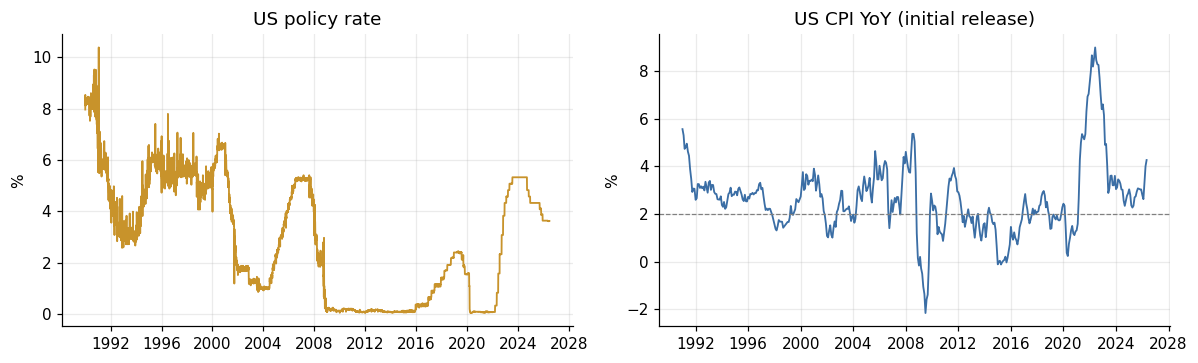
\includegraphics[width=\textwidth]{figs/data.png}
\caption{US policy rate and initial-release CPI year-over-year, 1990--2026. Using
the revised CPI instead of the initial release would leak information unavailable
at decision time.}
\label{fig:data}
\end{figure}

\section{The out-of-sample test}
At each month I refit the chain on past-only data and predict the distribution of
the next move, scoring mean log-loss (lower is better) against a climatology
baseline (the unconditional marginal of moves) and the unconditional chain. The
first-order chain beats climatology ($1.071$ vs.\ $1.162$ for the US), confirming
genuine predictive content. But \emph{raw} CPI conditioning is \emph{worse}
($1.136$): with the non-hold transitions split across five regimes, each
regime-row is estimated from a handful of observations and the variance swamps any
signal.

\section{The fix: shrinkage}
If the failure is variance, the remedy is shrinkage. I place a Dirichlet prior on
each regime row centered on the pooled (unconditional) row with strength $\tau$
pseudo-counts,
\[
\hat{p}(j \mid i, r) \;=\; \frac{c_{r,i,j} + \tau\, \bar{p}(j \mid i)}{n_{r,i} + \tau},
\]
so that $\tau \to 0$ recovers the raw conditional model and $\tau \to \infty$ the
unconditional one. A sweep (Figure~\ref{fig:tau}) shows a broad interior plateau,
$\tau \approx 20$--$500$, over which the shrunk conditional model \emph{beats the
unconditional chain}. The macro signal was real; it was drowned in variance, and
regularization recovered it.

\begin{figure}[t]
\centering
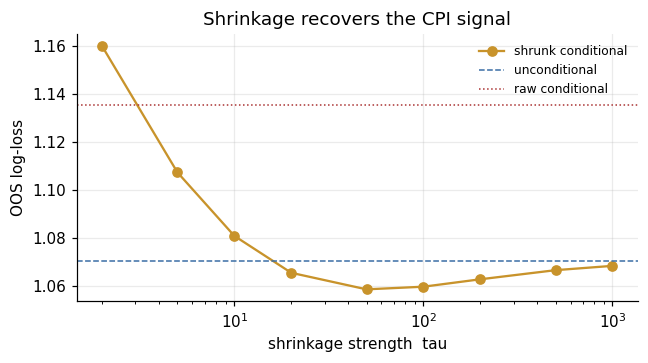
\includegraphics[width=0.62\textwidth]{figs/tausweep.png}
\caption{Out-of-sample log-loss of the shrunk conditional model versus shrinkage
strength $\tau$ (US). The shrunk model beats the unconditional chain over a broad
plateau, not a tuned point.}
\label{fig:tau}
\end{figure}

\section{Robustness}
\textbf{Replication.} The pattern---raw conditioning hurts, shrinkage helps---holds
in all three sovereigns (Table~\ref{tab:results}, Figure~\ref{fig:rep}).
\textbf{No tuned $\tau$.} A fully data-driven empirical-Bayes $\tau$, estimated
per-step from past-only data by maximizing the Dirichlet-multinomial marginal
likelihood, also beats the unconditional chain in all three with no tuning; it is
marginally worse than a fixed moderate $\tau$ only because it is conservative when
early data is thin, then adapts (settling near $130$ for the US, $300$ for the UK,
and $17$ for Germany---German decisions are the most regime-dependent).
\textbf{Cadence is not the lever.} Re-running at the Fed's roughly eight-meeting
annual cadence rather than monthly does not systematically help; even at meeting
frequency $60$--$80\%$ of decisions are holds, because policy is intrinsically
sticky.

\begin{table}[t]
\centering
\small
\begin{tabular}{lccc}
\toprule
Model (out-of-sample mean log-loss) & US & UK & Germany \\
\midrule
climatology & 1.162 & 1.010 & 0.615 \\
unconditional chain & 1.071 & 0.843 & 0.596 \\
conditional, raw & 1.136 & 0.904 & 0.662 \\
\textbf{conditional, shrunk ($\tau{=}50$)} & \textbf{1.059} & \textbf{0.819} & \textbf{0.549} \\
conditional, empirical-Bayes $\tau$ & 1.065 & 0.843 & 0.563 \\
\bottomrule
\end{tabular}
\caption{Out-of-sample mean log-loss (lower is better). Raw conditioning is worse
than the unconditional chain everywhere; the shrunk and empirical-Bayes versions
are better everywhere.}
\label{tab:results}
\end{table}

\begin{figure}[t]
\centering
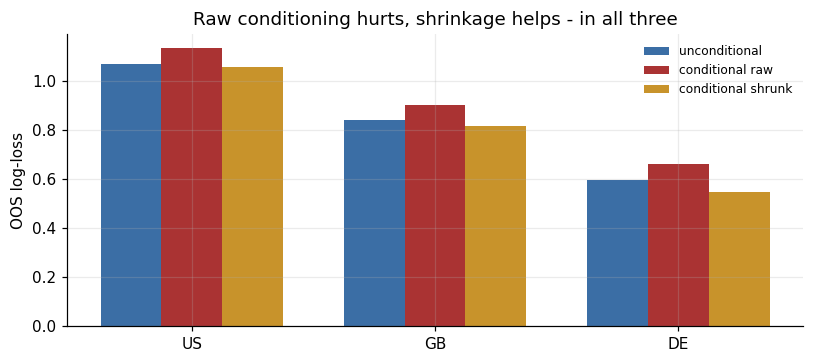
\includegraphics[width=0.78\textwidth]{figs/replication.png}
\caption{The flip replicates: raw conditioning hurts and shrinkage helps in the
US, UK, and Germany.}
\label{fig:rep}
\end{figure}

\section{From a forecast to a strategy}
A calibrated forecast is not yet money. Turning the model's expected move into a
duration tilt (expect cuts, lengthen duration; expect hikes, shorten) and pricing
the realized return off the actual Treasury curve, the timing strategy does
\emph{not} beat a constant two-year bond risk-adjusted (Sharpe $\approx 1.06$ vs.\
$1.39$; Figure~\ref{fig:bt}). It tilts long-duration only about $7\%$ of the time,
and those tilts add volatility without enough return. The forecasting edge is real
but lives in calibration, not in this simple tradeable rule.

\begin{figure}[t]
\centering
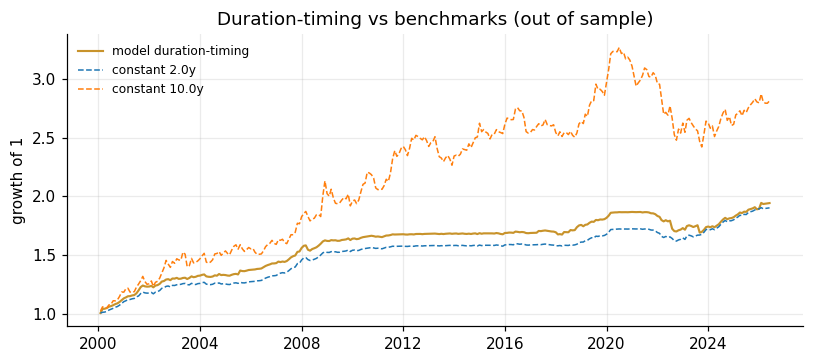
\includegraphics[width=0.78\textwidth]{figs/backtest.png}
\caption{Out-of-sample growth of \$1: the model's duration-timing strategy versus
constant-duration benchmarks. The strategy does not beat the constant two-year
bond risk-adjusted.}
\label{fig:bt}
\end{figure}

\section{Conclusion}
A memoryless Markov chain on Fed moves beats climatology out of sample; naive
inflation conditioning overfits; empirical-Bayes shrinkage recovers a small,
consistent, cross-country edge; cadence is not the lever; and the edge is in
calibration rather than a tradeable strategy. Every result is reproducible from a
seed under strict no-look-ahead with point-in-time CPI, and the honest negatives
are part of the finding. Natural extensions are the exact published FOMC calendar
(to settle the cadence question), a term-structure factor model for the curve, and
a richer mapping from forecast to position.

\vspace{4pt}
\noindent\footnotesize\textcolor{gray}{Code, the executable research notebook, and
this paper: \texttt{github.com/tanishhky/RateWalk}. Research software, not
investment advice.}

\end{document}
